\documentclass[journal]{IEEEtran}

\usepackage{cite}
\usepackage{amsmath,amssymb,amsfonts}
\usepackage{algorithmic}

\usepackage{graphicx}
\graphicspath{{../../Dissertacao/figuras/}}

\usepackage{textcomp}
\usepackage{xcolor}
\usepackage{booktabs}                        % AAB inserido
\usepackage[utf8]{inputenc}                  % AAB inserido
\usepackage{rotating}                        % AAB inserido

\usepackage{bbm}
\usepackage[binary-units]{siunitx}

\usepackage[caption=false,font=footnotesize]{subfig}
\DeclareMathOperator{\traco}{tr}



\begin{document}
\title{Fusion of Evidences in Intensities Channels for Edge Detection in PolSAR Images}
\author{Anderson A.\ de Borba, Maurício Marengoni, and Alejandro C.\ Frery,~\IEEEmembership{Senior Member,~IEEE}%
\thanks{A.\ A.\ de Borba is with the Dept.\ Engenharia Elétrica e Computação, Universidade Presbiteriana Mackenzie (UPM), and with IBMEC-SP, São Paulo, Brazil. anderson.borba@ibmec.edu.br}
\thanks{M.\ Marengoni is with the Dept.\ Engenharia Elétrica e Computação,
UPM, São Paulo, Brazil. mauricio.marengoni@mackenzie.br}
\thanks{A.\ C.\ Frery is with the Laboratório de Computação Científica e Análise Numérica (LaCCAN), Universidade Federal de Alagoas (UFAL), Maceió, Brazil. acfrery@laccan.ufal.br}}

\maketitle

\begin{abstract}
Synthetic Polarimetric Aperture Radar (PolSAR) sensors have reached an essential position in the area of remote sensing. 
The images coming from PolSAR sensors have speckle noise, making their processing and analysis challenging tasks. 
The present study discusses a detection method based on the fusion of evidence obtained in the intensity (hh), (hv), and (vv) channels of PolSAR multi-look images. 
The method consists of detecting transition points in the thinnest range of data that covers two regions using the maximum likelihood with estimates parameters from the Wishart distribution. 
The fusion methods used are the simple average, the discrete wavelet (DWT), and stationary (SWT) transform, the principal component analysis (PCA), the ROC statistic, and a multi-resolution method based on singular values (MSVD). 
The results indicate an assessment of the influence of each intensity channel in the fusion of evidence with possible paths for future research.
\end{abstract}

\begin{IEEEkeywords}
PolSAR, edge detection, maximum likelihood estimation, fusion methods. 
\end{IEEEkeywords}

\section{Introduction}\label{sec_01}
\IEEEPARstart{P}{olarimetric} synthetic aperture radar (PolSAR) has achieved an essential position as a remote sensing method. This area require specifically tailored signal processing techniques, then a method for detection and fusion of edge evidence is presented. 

Among the available edge detection techniques for SAR and PolSAR images, it is worth mentioning:
\begin{itemize}
\item techniques based on denoising~\cite{sjx, lzly, wxbzw, law, cgaf} used to PolSAR image;   
\item the Markov random fields~\cite{bf} method applied to SAR images;	
\item the deep learning approach~\cite{bac, ztmxzxf} applied to segmentation and classification in PolSAR / SAR image; and,
\item statistical techniques~\cite{gmbf, fbgm, nhfc} applied in edge detection in PolSAR / SAR image.
\end{itemize}
%\IEEEPARstart{W}{e present}
%results on the detection and fusion of edge evidence applied to Polarimetric Synthetic Aperture Radar (PolSAR) images.
%
%Among the available edge detection techniques for SAR and PolSAR images, it is worth mentioning:
%\begin{itemize}
%\item techniques based on denoising~\cite{sjx, lzly, wxbzw, law, cgaf};   
%\item methods that use Markov random fields~\cite{bf};	
%\item the deep learning approach~\cite{bac, ztmxzxf}; and,
%\item statistical techniques~\cite{gmbf, fbgm, horrit}.
%\end{itemize}

This article follows the statistical modeling approach using the techniques described in~\cite{gmbf, fbgm, nhfc} to find edge evidence, as well as, the process for fusing this information is described in~\cite{mit, bmf_2019}. The technique used does not attempt to eliminate the existing speckle noise, but to extract information from its statistical properties.

% The images PolSAR are contaminated with speckle noise giving the image a granular appearance, and its multiplicative nature makes analyzing the images a challenging task. 

An estimation of the the probability density function (PDF) parameters is performed by log-likelihood maximum method, and the BFGS optimization method implemented in the maxLik package~\cite{ht} is used to found the parameters.

The parameters are applied to generate the log-likelihood function to find the transition point between two samples; this function is non-differentiable at various points in the domain. It is known that classical methods have difficulties in finding the maximum of a non-differentiable function. The Generalized Simulated Annealing (GenSA)~\cite{xgsh} method solves this problem. 
 
Further, the present work presenting two fusion methods, the methods DWT~\cite{n_r} and SVD~\cite{naidu}. It aims to show the feasibility of a procedure for edge detection in PolSAR images. The objective is to understand and quantify the importance of the information provided by each channel to improve the edge detection process.

The article is structured as follows.
Section~\ref{sec_02} describes statistical modeling.
Section~\ref{sec_03} describes edge detection for PolSAR data.
Section~\ref{sec_04} describes the approach to edge evidence fusing.
Section~\ref{sec_05} presents the numerical results.
Finally, Section~\ref{sec_06} concludes the work with observations, future directions of research, and the feasibility of detecting edges in each channel of PolSAR images.

\section{Statistical modeling for PolSAR data}\label{sec_02}
Multi-looked fully polarimetric data follow the Wishart distribution with PDF defined by:
\begin{equation}
    f_{\mathbf{Z}}(\mathbf{Z};\mathbf{\Sigma},L)=\frac{L^{mL}|\mathbf{Z}|^{L-m}}{|\mathbf{\Sigma}|^{L}\Gamma_m(L)} \exp(-L\traco(\mathbf{\Sigma}^{-1}\mathbf{Z})),
    \label{eq_04}
\end{equation} 
where, $\traco(\cdot)$ is the trace operator of a matrix, $\Gamma_m(L)$ is a multivariate Gamma function defined by
\begin{equation*}
	\Gamma_m(L)=\pi^{\frac{1}{2}m(m-1)} \prod_{i=0}^{m-1}\Gamma(L-i),
\end{equation*}
and $\Gamma(\cdot)$ is the Gamma function.
In this study, $m=3$ is used. 
This situation is denoted by $\mathbf{Z}\sim W(\mathbf{\Sigma}, L)$, which satisfies $E[\mathbf{Z}]=\mathbf{\Sigma}$. 
This assumption usually holds on targets where the speckle is fully developed.

\section{Edge Detection}\label{sec_03}
%The noise in these kinds of images is multiplicative, making edge detection in PolSAR images a challenging task. 
The main idea for edge detection is based in~\cite{gmbf, fbgm, nhfc} and show how to detect the transition point in a thin strip between two regions of the image. The transition point is considered as edge evidence. 

The following procedure is proposed:
\begin{enumerate}
	\item Identify the centroid of a region of interest (ROI) in an automatic, semi-automatic or manual manner;
	\item casting radial line from the centroid to the outside of the area;
	\item collect data around the radial lines using the  Bresenham's midpoint line algorithm, ideally of the size of a pixel;
	\item detect points in the data strips which provide evidence of changes in their statistical properties, i.e., a transition point;
	\item use the GenSA method,~\cite{xgsh}, to find maximum points in the functions of interest;
	\item fuse the evidence of detected edges in the (hh), (hv) and (vv) channels.
\end{enumerate}

The Maximum Likelihood Estimator (MLE) method found in~\cite{gmbf, nhfc} is used to detect transition points described in item (4) above. Thus, for each radial line of a ROI, a data range is considered,

\begin{equation}\nonumber
	z = (z_1,z_2,\dots,z_N)
\end{equation}
with partition represented by
\begin{equation}\label{func_max_ver_uni_gamma} 
\begin{array}{lll}
	Z_k&\sim& f_Z(z_k;\mu_\text{I},L_\text{I}), k=1,\dots,j\\
	Z_k&\sim& f_Z(z_k;\mu_\text{E},L_\text{E}), k=j+1,\dots,N
\end{array}
\end{equation}
where, for each $k$, $z_k$ is the realization of the random variable $Z_k$, and they are distributed according to their PDF. The indices I e E define if the point is internal (I) or external (E) of a ROI.

The Gamma model is used to estimate $(\mu_\text{I},L_\text{I})$ and $(\mu_\text{E},L_\text{E})$:
\begin{equation}\label{func_dens_uni_gamma}
	f_Z(z_k;\mu,L)=\frac{L^{L}z_k^{L-1}}{\mu^{L}\Gamma(L)} \exp\Big\{-L\frac{z_k}{\mu}\Big\}.
\end{equation}
Applying the natural logarithm on both sides of~\eqref{func_dens_uni_gamma}, and performing  the necessary algebra,  the function \eqref{func_max_ver_uni_gamma} is found
\begin{equation}\label{func_max_ver_uni_gamma}
\begin{split}
	\ln f_Z(z_k;\mu,L)&= L\ln L +(L - 1) \ln z_k-L \ln \mu \\
	 	                  &{}- \ln \Gamma(L) -\frac{L}{\mu} z_k.\\
\end{split}
\end{equation}

The function of maximum likelihood $\ell$ is considered for each partition of the data:
\begin{equation}\nonumber
\ell(j;\mu, L)=\sum_{k=1}^{j}\ln f_{Z}(z_k;\mu,L)
             +\sum_{k=j+1}^{N}\ln f_{Z}(Z_k;\mu,L).
\end{equation}
 
Using~\eqref{func_max_ver_uni_gamma} and performing the necessary algebra, the resulting equation is 
\begin{equation}\label{func_l_param}
  \ell(j;\mu, L)=j\ell_1(\mu, L) + (N - j)\ell_2(\mu, L),
 \end{equation}
where
\begin{equation}\label{func_l_param_1_2}
\begin{split}
    \ell_1(\mu, L)&=L\ln L+\frac{L-1}{j}\sum_{k=1}^{j}\ln z_k-L\ln\mu\\
    &{}-\ln\Gamma(L) -\frac{L}{j\mu}\sum_{k=1}^{j} z_k,\text{ and}\\
    \ell_2(\mu, L)&=L\ln L+\frac{L-1}{N-j}\sum_{k=j+1}^{N}\ln z_k-L\ln\mu\\
    &{}-\ln\Gamma(L) -\frac{L}{(N-j)\mu}\sum_{k=j+1}^{N} z_k.
 \end{split}
\end{equation}
 
The functions defined in~\eqref{func_l_param_1_2} are used to estimate the parameters $(\mu, L)$ by solving the following optimization problems 
\begin{equation}\label{optimiz_l_1}
(\widehat{\mu}_\text{I},\widehat{L}_\text{I})= \arg\max\limits_{(\mu,L)\in \mathrm{R}^{+}\times\mathrm{R}^{+}}\ell_1(\mu,L),
\end{equation}
and
\begin{equation}\label{optimiz_l_2}
(\widehat{\mu}_\text{E},\widehat{L}_\text{E})= \arg\max\limits_{(\mu,L)\in \mathrm{R}^{+}\times\mathrm{R}^{+}}\ell_2(\mu,L).
\end{equation} 

The BFGS optimization method implemented in the maxLik package~\cite{ht} to estimate $(\widehat{\mu}_I, \widehat{L}_I)$ and $(\widehat{\mu}_E, \widehat{L}_E)$, for every $j$ in the data strip is used.

As the parameters $(\widehat{\mu}_I, \widehat{L}_I)$ and $(\widehat{\mu}_E, \widehat{L}_E)$ are known, the $\ell$ function based on~\eqref{func_l_param} is constructed as follows,
\begin{equation}\label{l_com_paremetros}
 \begin{split}
\ell&(j;\widehat{\mu}_I, \widehat{L}_I,\widehat{\mu}_E, \widehat{L}_E)=j\Bigg[  \widehat{L}_I(\ln \widehat{L}_I -\ln \widehat{\mu}_I) \\
                                          &{}- \ln \Gamma(\widehat{L}_I) + \frac{\widehat{L}_I  - 1}{j} \sum_{k=1}^{j}  \ln z_k -\frac{\widehat{L}_I}{j\widehat{\mu}_I} \sum_{k=1}^{j}   z_k\Bigg] \\
                                   &{}+(N-j)\Bigg[\widehat{L}_E(\ln \widehat{L}_E - \ln \widehat{\mu}_E)\\
                                   &{}-\ln \Gamma(\widehat{L}_E) + \frac{\widehat{L}_E - 1}{N-j} \sum_{k=j+1}^{N}\ln z_k
                                   -\frac{\widehat{L}_E}{(N-j)\widehat{\mu}_E} \sum_{k=j+1}^{N}z_k\Bigg]. \\
 \end{split}
 \end{equation}
 
The GenSA is used to find  
$$
\widehat{\jmath}= \arg\max\limits_{j\in [\min_s,N-\min_s]}\ell(j;\widehat{\mu}_I, \widehat{L}_I,\widehat{\mu}_E, \widehat{L}_E),
$$ 
where $\min_s$ is a minimum sample size that we set to $14$.

\section{Methods of fusion of edge evidence}\label{sec_04}

 The simple average, stationary wavelet transform (SWT), principal components analysis PCA, and ROC statistics fusion methods are summarized in~\cite{bmf_2019}, more details in~\cite{n_r,mit,gs}, and~\cite{fawcett}. The multi-resolution discrete wavelet transform and multi-resolution singular value decomposition (MSVD) fusion methods are presented bellow.

\subsection{Multi-Resolution Discrete Wavelet Transform DWT Fusion~\cite{n_r}}  
The filters DWT are applied separately in vertical and horizontal directions and down-sampled by a factor of two in image I. In this way, the image is filtered by the low pass filter L in the vertical direction and the high pass filter H in the horizontal direction and then down-sampled by a factor of two to create the coefficients matrices $\text{I}_\text{L}$ and $\text{I}_\text{H}$. After this, the decomposition $\text{I}_\text{L}$ and $\text{I}_\text{H}$ are submitted to the low pass and high pass filters again  in both direction and newly down-sampled by a factor of two to create sub-images named $\text{I}_\text{LL}$,$\text{I}_\text{LH}$, $\text{I}_\text{HL}$ and $\text{I}_\text{HH}$. The successive levels of decomposition can be achieved by repeating this procedure.

The DWT fusion method for each channel has following steps:
\begin{enumerate}
\item Calculate the DWT decomposition by getting $\text{I}_\text{HH}$, $\text{I}_\text{HL}$, $\text{I}_\text{LH}$ and $\text{I}_\text{LL}$ for each channel;
\item in the decomposition $\text{I}_\text{HH}$, the arithmetic mean of all channels is computed, pixel by pixel, and in the decomposition $\text{I}_\text{HL}$, $\text{I}_\text{LH}$, and $\text{I}_\text{LL}$, the maximum is found among all channel, pixel by pixel, finding a new operators $\bar{\text{I}}_\text{HH}$, $\bar{\text{I}}_\text{HL}$, $\bar{\text{I}}_\text{LH}$, and $\bar{\text{I}}_\text{LL}$;
\item the image with the fusion of edge evidence IF(x, y) is computed performing the inverse DWT transformation to operators $\bar{\text{I}}_\text{HH}$, $\bar{\text{I}}_\text{HL}$, $\bar{\text{I}}_\text{LH}$, and $\bar{\text{I}}_\text{LL}$.
\end{enumerate}

\subsection{Multi-Resolution Singular Value Decomposition SVD Fusion - MSVD~\cite{naidu}}
Multi-Resolution Singular Value Decomposition SVD Fusion works similar to the DWT method. The difference consists in changing the DWT filters by the SVD filters. The SVD fusion method can be summarized for each channel, as follows:
\begin{enumerate}
\item Organize the data in matrices $X_\ell$ with dimension $4\times\text{MN}$ according to~\cite{naidu}. Where M is the number of rows and N is the number of columns in the PolSAR image, and $\ell$ is the level resolution to set;  
\item find the SVD decomposition to matrix $T=X_\ell X_\ell^T=U_\ell S^2 U_\ell^T$, where $s(1)\geq s(2) \geq s(3) \geq s(4)$ compose the singular value matrix $S$, and $U$ is an real or complex unitary matrix;
\item put $\widehat{X}_\ell=U_\ell^TX_\ell$ and transform the lines on this matrix in new matrices with dimensions $\frac{\text{M}}{2}\times\frac{\text{N}}{2}$, named respectively $\{\Phi_\ell, \Psi_\ell^\text{V}, \Psi_\ell^\text{H}, \Psi_\ell^\text{D}\}$. In the next level decomposition, the $\widehat{X}_\ell$ is replaced by $\Phi_\ell$ until the level L is reached. The MSVD method is represented as:
\begin{equation}\label{msvd_iter}
\widehat{X}\leftarrow \left\{\Phi_L,\{\Psi_\ell^\text{V},\Psi_\ell^\text{H},\Psi_\ell^\text{D} \}_{\ell=1}^L,\{U_\ell\}_{\ell=1}^L \right\}
\end{equation}
\item once the MSVD is applied to level $\ell$ the fusion process is executed as follow: In the operators $\Phi_\ell^\text{V}$, $\Phi_\ell^\text{H}$ and $\Phi_\ell^\text{D}$, the maximum is found among all channel, pixel by pixel, resulting in new operators $\bar{\Phi}_\ell^\text{V}$, $\bar{\Phi}_\ell^\text{H}$ and $\bar{\Phi}_\ell^\text{D}$. The other operators $\Psi_\ell$, and $U_\ell$, are averaged over all the channels. See~\cite{naidu} for details;
\item the image with the fusion of edge evidence $\text{IF}(x,y)$ is performed with the SVD transformation. 
\end{enumerate}
\section{Numerical results}\label{sec_05}

\subsection{Real PolSAR image}
The PolSAR image of the Flevoland region in the Netherlands is used for the numerical tests. 
Fig.~(\ref{flevoland_radial_4look}) shows the ROI, with the radial lines for edge detection.

\begin{figure}[hbt]
\centering
	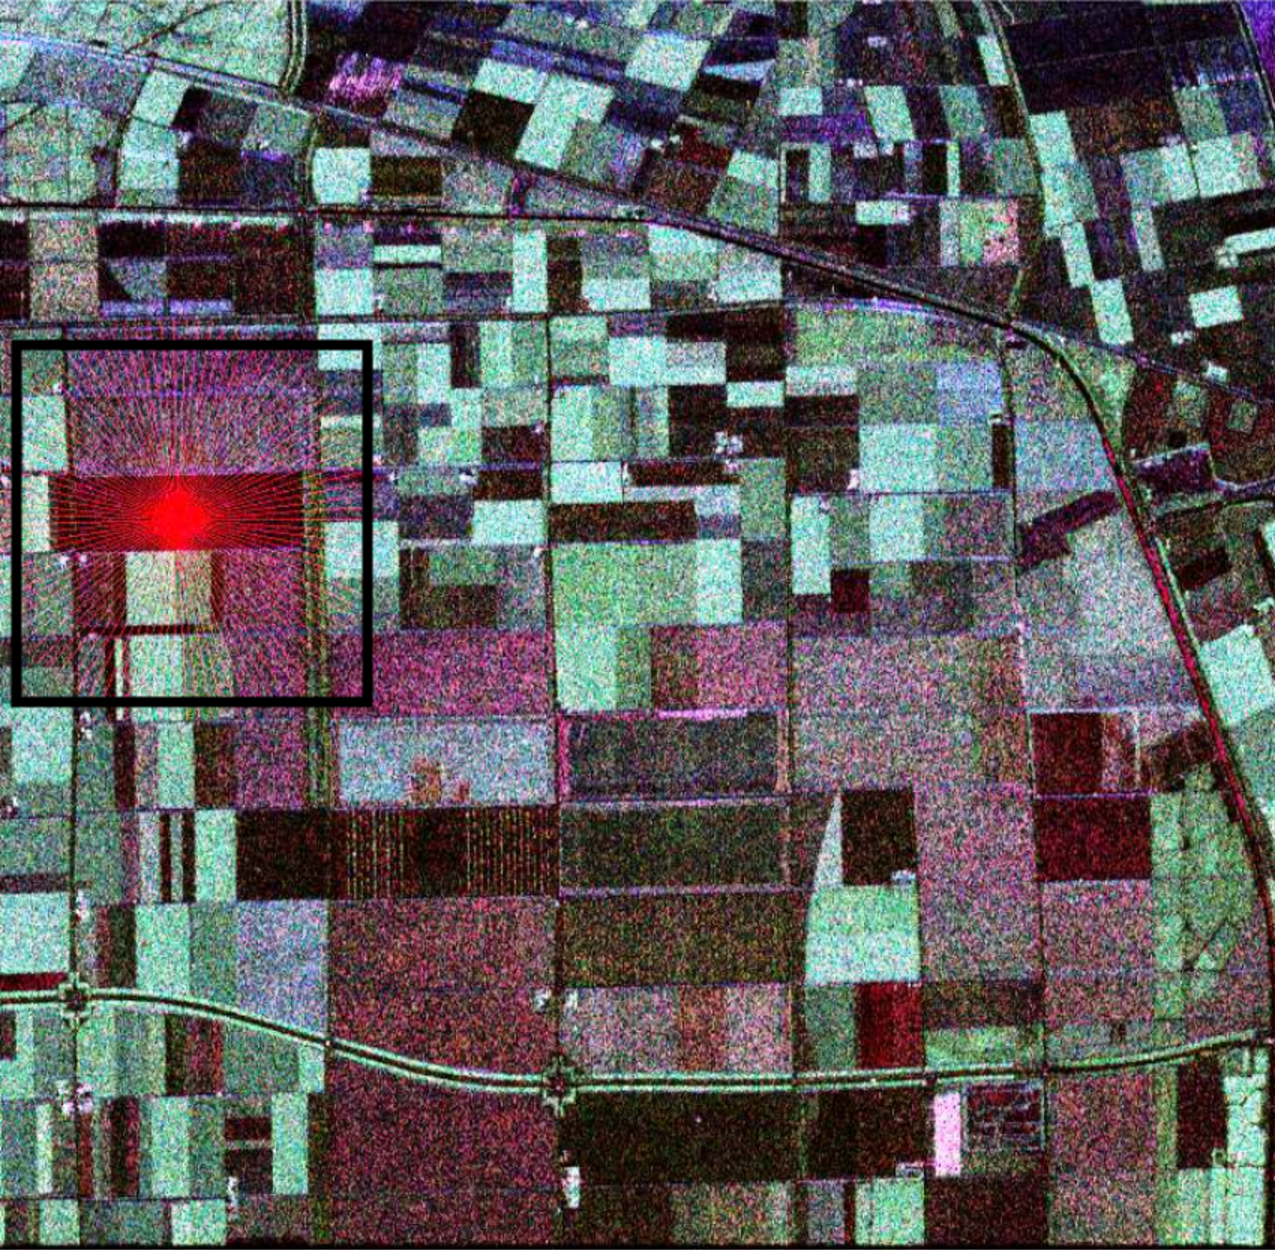
\includegraphics[width=\linewidth]{flevoland_radial_4_look_black}
	\caption{ROI in the image of Flevoland.}
\label{flevoland_radial_4look}
\end{figure}

The estimates from equations~\eqref{optimiz_l_1} and~\eqref{optimiz_l_2} are used in equation~\eqref{l_com_paremetros} generating an oscillation at the end of each radial line, depending on the radial considered. In order to get around this problem, in this PolSAR image, 14 pixels on each side of radial lines were not considered. The number of pixel were determined empirically.

Figs.~\ref{evidencias_hh_hv_vv}\subref{evidencias_hh_hv_vv:a}, \subref{evidencias_hh_hv_vv:b} and~\subref{evidencias_hh_hv_vv:c} show, respectively, the edge evidence in the $\text{hh}$, $\text{hv}$ and $\text{vv}$ channels. For each of these images, the MLE is executed.

It is worth noting that GenSA has accurately identified the maximum value of function $\ell(j)$, even in the presence of multiple local maxima. Another important observation concerns the performance of the proposed method in the $\text{hv}$ channel. The method presents a few outliers points, and, good accuracy in the detection edges evidence. The method presents the best performance when compared to channels $\text{hh}$ and $\text{vv}$. 
   \begin{figure*}[hbt]
	\centering
     \subfloat[Evidences in channel $\text{hh}$ \label{evidencias_hh_hv_vv:a}]{%
       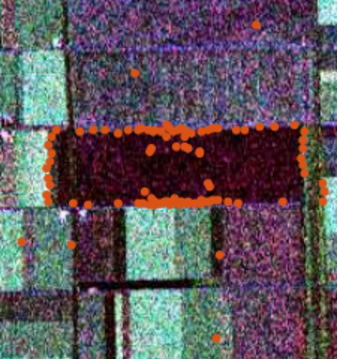
\includegraphics[width=0.32\linewidth]{flevoland_hh_evid_param_L_mu_14_pixel_crop}
     }
     \subfloat[Evidences in channel $\text{hv}$ \label{evidencias_hh_hv_vv:b}]{%
       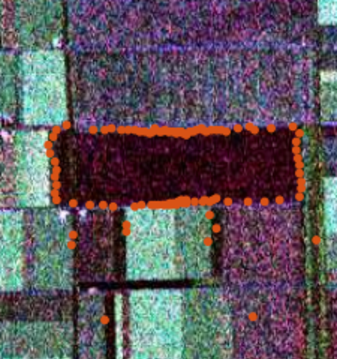
\includegraphics[width=0.32\linewidth]{flevoland_hv_evid_param_L_mu_14_pixel_crop}
     }
     \subfloat[Evidences in channel $\text{vv}$ \label{evidencias_hh_hv_vv:c}]{%
       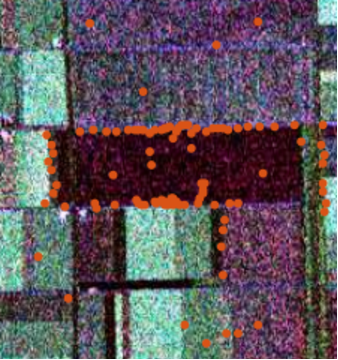
\includegraphics[width=0.32\linewidth]{flevoland_vv_evid_param_L_mu_14_pixel_crop}
     }
     \caption{Edges evidences 14 pixel range}
     \label{evidencias_hh_hv_vv} 
   \end{figure*}

Figs.~\ref{fusion_met}\subref{fusion_met:a},~\subref{fusion_met:b},~\subref{fusion_met:c},~\subref{fusion_met:d},~\subref{fusion_met:e}, and~\subref{fusion_met:f} show the results of fusing these evidences. 

The simple average and PCA methods have similar performances to indicate pixels as edges. The time to perform the methods is shown in the table~(\ref{metrica_de_tempo}). Thus, one can see that the time for the PCA method is 2.19 times longer than the simple average.  

The MSVD method shows excellent performance to indicate pixels of edges; the number of pixels outliers is much smaller than the other methods. The significant disadvantage of the MSVD method is the runtime. Table~(\ref{metrica_de_tempo}) shows that it has the highest time.

The ROC Fusion shown edge pixels with good accuracy and a small number of outliers, but it doesn't show pixels that are edges. One way to get around this problem would be to increase the number of channels considered using other PDF.

The post-processing is an option to be used in all the fusion methods. An idea can be found in Ref.~\cite{gmbf}. 

\begin{figure*}[hbt]
	\centering
     \subfloat[Average fusion\label{fusion_met:a}]{%
       %\includegraphics[width=0.2\textwidth]{example-image-a}
       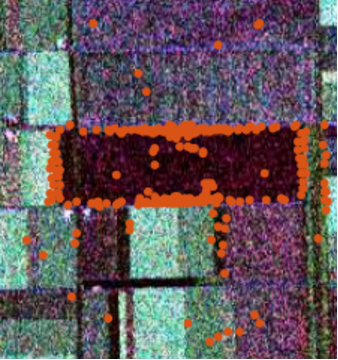
\includegraphics[width=0.32\linewidth]{flevoland_fus_media_param_L_mu_14_pixel_crop}
     }
     \subfloat[SWT fusion\label{fusion_met:b}]{%
       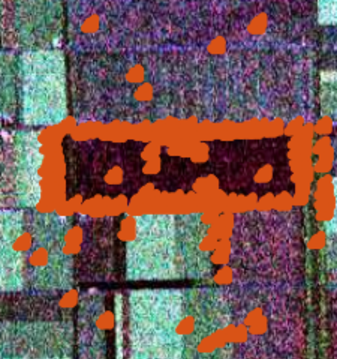
\includegraphics[width=0.32\linewidth]{flevoland_fus_swt_param_L_mu_14_pixel_crop}
     }
     \subfloat[PCA fusion \label{fusion_met:c}]{%
       %\includegraphics[width=0.2\textwidth]{example-image-a}
       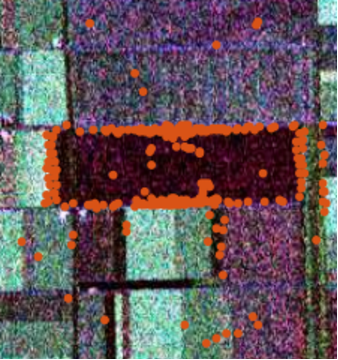
\includegraphics[width=0.32\linewidth]{flevoland_fus_pca_param_L_mu_14_pixel_crop}       
     }\\
     \subfloat[ROC fusion\label{fusion_met:d}]{%
       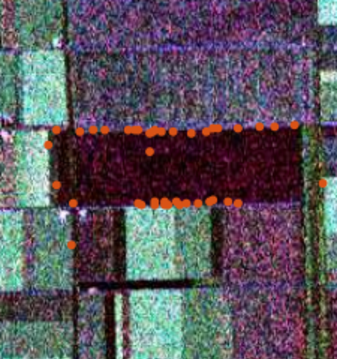
\includegraphics[width=0.32\linewidth]{flevoland_fus_roc_param_L_mu_14_pixel_crop}
     }
     \subfloat[DWT fusion\label{fusion_met:e}]{%
       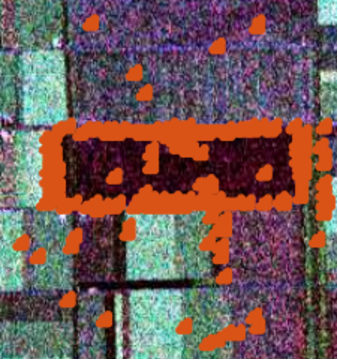
\includegraphics[width=0.32\linewidth]{flevoland_fus_dwt_param_L_mu_14_pixel_crop}
     }
     \subfloat[MSVD fusion\label{fusion_met:f}]{%
       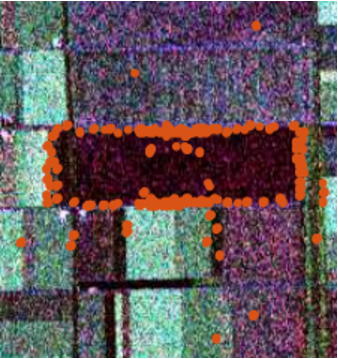
\includegraphics[width=0.32\linewidth]{flevoland_fus_svd_param_L_mu_14_pixel_crop}
     }
     \caption{Fusion methods}
     \label{fusion_met}
\end{figure*}

\subsection{Implementation Details}
The system presented here was executed on a Intel\copyright\ Core i7-9750HQ CPU \SI{2.6}{\giga\hertz} \SI{16}{\giga\byte} RAM computer.  
The method for detecting edge evidence MLE was implemented in R language; on the other hand, the fusion methods were implemented in Matlab language. 
Table~\ref{metrica_de_tempo} shows the computational cost of each of the fusion methods.

\subsection{Processing times} 

This section presents a table of the processing time to fusion's methods. The measurement of time was performed only for the fusion method, disregarding the time for the method that finds the evidence of edges, because it is the same for all fusion methods. The measurement was performed by running the fusion method 20 times and performing the average of these times. The result is shown in the first row of the table (\ref{metrica_de_tempo}), the second row of the table  (\ref{metrica_de_tempo}) was constructed by choosing the shortest time of the methods as the reference time (TR) that shows how longer the others methods are.
\begin{table}[hbt]
	\centering
	\tiny
	\caption{System performance.}\label{metrica_de_tempo}
\begin{tabular}{@{}lllllll@{}} \toprule
	Method       & Average    &   PCA      &  ROC      & DWT       &  SWT        &  MSVD \\ \midrule
	Time (s)      & 0.00858185 & 0.01880955 &0.39989020 &0.07938820 &  0.18071635 & 1.11195710  \\
    Ref. time     & TR & 2.19TR &46.59TR & 9.25TR   & 21.05TR & 129.57TR  \\ \bottomrule
\end{tabular}
\end{table}
\section{Conclusion}\label{sec_06}

Initially, evidence of edges was found using the maximum likelihood method and BFGS to estimate the $L$ and $\mu$ parameters. Later this parameter was used in the maximum likelihood method; at this point, the GenSA method for estimation of edge evidence were applied. In the article, three intensity channels are used to apply the maximum likelihood methods showing excellent accuracy on the actual image of a Flevoland region. The maximum likelihood method in the (hv) channel has superior performance compared to (hh) and (vv) channels.

It is essential to point out that the maximum likelihood method when inserting the $L$ and $\mu$ parameters results in a non-smooth function presenting many local maxima. The difficulty of using the classical optimization methods in this kind function is known, then to get around this problem the simulated annealing method was applied because it is appropriate to optimize non-differentiate functions.

The fusion methods like simple average, SWT, PCA, ROC, DWT, and MSVD were applied to the results of the maximum likelihood methods on each channel. The purpose of applying the fusion methods was to obtain better edge detection accuracy and measure the importance of each channel in the final fusion result. On this sense are can notice that mainly the (vv) channel did not contribute to get a good accuracy of the fusion methods.

From the obtained results, the feasibility of procedure proposes for edge detection in PolSAR images is shown.

Finally, three observations are highlighted on future work; the ROC statistic can be improved by increasing the number of PDF for the intensity channels, the weight adjustment for the channels or the choice of the best channels for the fusion of edge evidence, and the use of post-processing on the images coming from the fusion.

\bibliographystyle{IEEEtran}
\bibliography{../../../Text/bibliografia}
\end{document}

